\section{Introduction}
\label{sec:intro}

A common near-term design for quantum image classification feeds a convolutional network
into a small variational quantum circuit (VQC) that acts as the classifier head
\citep{mari2020}, building on variational quantum classifiers
\citep{mitarai2018,havlicek2019,benedetti2019,cerezo2021}. When the network is trained jointly
\emph{through} the circuit, the head does more than classify: its gradients shape the
features the backbone learns. A comparison between a quantum head and a classical one
therefore compares two things at once, the heads and the representations they induce.
The question reaches beyond quantum machine learning: a head that distorts the features
trained through it is a known failure mode of fine-tuning \citep{kumar2022}, and here the
distortion turns out to track a structural quantity that can be computed before training.
Benchmarks of quantum classifiers typically score accuracy on fixed inputs
\citep[e.g.][]{fulton2026,slattery2022}; \citet{bowles2024} also replace the quantum layer of a trained
dressed hybrid network with a classical one and visualize how the learned layers transform
the data. Controls that isolate a circuit inside a hybrid model score predictive performance
\citep{kolle2024,elhag2026}. To our knowledge, none of these measures quantitatively what the quantum head
does to the representation trained through it, or which part of the circuit is
responsible.

We answer both questions for a CNN with an 8-dimensional bottleneck and an 8-qubit head
built from angle encoding $R_y(\pi\tanh z_j)$, four layers of trainable rotations each
followed by a ring of CNOTs, and a linear readout of $\ZZ{k}$. After joint training we
freeze each backbone and fit the same linear probe to its bottleneck, so that probe
accuracy compares the representations directly. The default VQC head lowers this probe
accuracy, and the size of the drop follows the circuit's CNOT structure. An exact identity
defines a structural descriptor whose order tracks this cost: when every trainable rotation
is zero, which is near where
training starts, each readout is
$\ZZ{k}=\prod_{j\in S_k}\cos(\pi\tanh z_j)$, a product of cosines over a set $S_k$ of
inputs fixed by the CNOT layers alone (\cref{fig:hero}a). The mean size of these sets, the
\emph{product order}, is 1 without CNOTs, 2.5 for the default circuit and 5.25 when a
single ring follows the last layer.

% Fig 1 (hero); panels (a, grids) and (b) from scripts/gen_fig1*.py, schematic drawn in fig1a_schematic.tex
\begin{figure*}[t]
  \centering
  % Fig 1a schematic: CNN -> bottleneck z -> 8-qubit VQC head -> linear readout, and the common
% linear probe on the frozen bottleneck. Requires tikz with positioning, arrows.meta, fit,
% shapes.geometric.
\begin{tikzpicture}[
    x=1cm, y=1cm, font=\footnotesize,
    box/.style={draw, rounded corners=1.5pt, minimum height=6mm, inner sep=2.5pt, align=center},
    gate/.style={draw, fill=white, minimum height=4.4mm, minimum width=9mm, inner sep=1pt, font=\scriptsize},
    arr/.style={-{Stealth[length=1.6mm]}, semithick},
  ]
  % classical front end
  \node[box] (img) at (0, 0) {image};
  \node[box, trapezium, trapezium angle=70, shape border rotate=270, minimum width=8mm] (cnn) at (1.45, 0) {CNN};
  \node[box] (z) at (2.95, 0) {$z\in\mathbb{R}^8$};
  \draw[arr] (img) -- (cnn);
  \draw[arr] (cnn) -- (z);
  \draw[arr] (z.east) -- (3.95, 0);

  % qubit wires q0, q1, ..., q7
  \foreach \y/\lab in {0.62/q_0, 0.22/q_1, -0.62/q_7} {
    \draw[thin] (4.55, \y) -- (10.0, \y);
    \node[font=\scriptsize, anchor=east] at (4.55, \y) {$\lab$};
  }
  \foreach \x in {5.15, 6.75, 9.45} \node[font=\scriptsize] at (\x, -0.18) {$\vdots$};

  % encoding R_y(a_j)
  \foreach \y/\j in {0.62/0, 0.22/1, -0.62/7}
    \node[gate, fill=blue!6] at (5.15, \y) {$R_y(a_{\j})$};

  % one variational layer: R_y R_z on every qubit, then a CNOT ring; repeated L times
  \foreach \y in {0.62, 0.22, -0.62}
    \node[gate] at (6.75, \y) {$R_y R_z$};
  \fill (7.65, 0.62) circle (1.3pt);                       % CNOT(0 -> 1)
  \draw (7.65, 0.62) -- (7.65, 0.22);
  \draw (7.65, 0.22) circle (2.6pt); \draw (7.65, 0.13) -- (7.65, 0.31);
  \fill (8.0, 0.22) circle (1.3pt);                        % CNOT(1 -> 2), down the ring
  \draw (8.0, 0.22) -- (8.0, -0.08);
  \node[font=\scriptsize] at (8.0, -0.2) {$\cdots$};
  \fill (8.4, -0.62) circle (1.3pt);                       % CNOT(7 -> 0) closes the ring
  \draw (8.4, -0.62) -- (8.4, 0.62);
  \draw (8.4, 0.62) circle (2.6pt); \draw (8.4, 0.53) -- (8.4, 0.71);
  \draw[dashed, rounded corners=2pt, gray] (6.15, -0.88) rectangle (8.65, 0.88);
  \node[font=\scriptsize, gray!70!black, anchor=north] at (7.4, -0.9) {$\times L$; CNOT layout varied};

  % measurement
  \foreach \y/\k in {0.62/0, 0.22/1, -0.62/7}
    \node[gate, minimum width=8mm] at (9.45, \y) {$\langle Z_{\k}\rangle$};

  % head frame and readout
  \node[draw, dashed, rounded corners=3pt, fit={(3.95, 1.0) (9.95, -1.25)}, inner sep=1pt,
        label={[font=\scriptsize, anchor=south west]north west:VQC head, 8 qubits}] (head) {};
  \node[box, anchor=west] (lin) at (10.75, 0) {Linear};
  \draw[arr] (10.0, 0) -- (lin.west);

  % zero-rotation identity
  \node[font=\scriptsize, anchor=west] at (4.25, -1.65)
    {$a_j=\pi\tanh z_j$;\ \ at zero variational rotations
     $\langle Z_k\rangle=\prod_{j\in S_k}\cos a_j$, with $S_k$ fixed by the CNOTs};

  % common linear probe on the frozen bottleneck
  \node[box, draw=gray, text=gray!70!black] (probe) at (2.55, -1.5) {common linear probe\\[-1pt](backbone frozen)};
  \draw[arr, dashed, gray] (z) -- (probe);
\end{tikzpicture}
\\[3mm]
  \begin{minipage}[c]{0.36\textwidth}
    \centering
    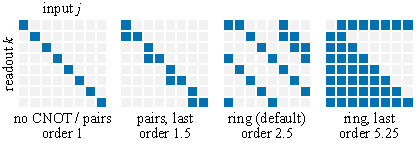
\includegraphics[width=\linewidth]{figures/fig1a_supports.pdf}\\[1mm]
    {\small (a)}
  \end{minipage}\hfill
  \begin{minipage}[c]{0.60\textwidth}
    \centering
    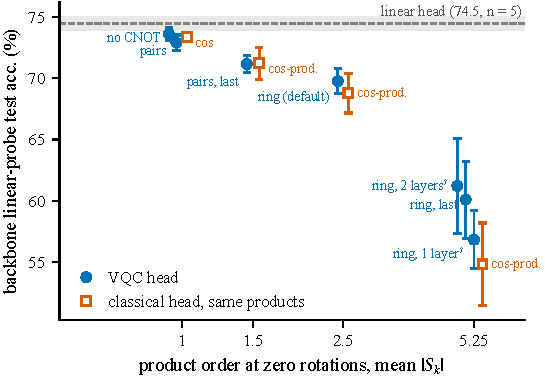
\includegraphics[width=\linewidth]{figures/fig1b_probe_vs_order.pdf}\\
    {\small (b)}
  \end{minipage}
  \caption{\textbf{(a)} A CNN feeds an 8-dimensional bottleneck $z$ into an 8-qubit VQC head
  (default: four $R_yR_z$ layers, each followed by a CNOT ring $(q, q{+}1 \bmod 8)$; variants
  place CNOTs after the last layer only (``last''), use $L\in\{1,2\}$ layers, or replace the ring
  by disjoint pairs $(0,1),(2,3),(4,5),(6,7)$). With every variational rotation at zero, each
  readout is exactly $\langle Z_k\rangle=\prod_{j\in S_k}\cos(\pi\tanh z_j)$; the grids mark
  $j\in S_k$ in blue (rows: readouts $k$, columns: inputs $j$). Pairs after every layer cancel
  at zero rotations, so their supports equal the no-CNOT ones. Product order is
  $\frac18\sum_k|S_k|$. The backbone is evaluated by one common linear probe on the frozen
  bottleneck. \textbf{(b)} CIFAR-10 with 4,000 training images: probe test accuracy against
  product order (log axis) for VQC heads (filled) and classical heads trained end to end on the
  zero-rotation products of a circuit (open; at order 5.25 these are the supports of ``ring,
  last'' and ``ring, 1 layer''; ``ring, 2 layers'' has different supports of the same mean
  order). Mean $\pm$ SD over 5 seeds ($\dagger$: 3); head learning rate selected on mean
  validation accuracy over seeds 0--2, seeds 3--4 run at that choice. Dashed line and band:
  linear head. Points at one order are offset horizontally. The plot shows an association;
  order co-varies with support overlap. Open diamonds: six CNOT layouts outside the ring family (5 seeds, \cref{app:family}),
  whose probe accuracy was predicted before training from the dotted fit over the ring-family (seeds 0--2)
  VQC circuits (linear in order, hence curved on the log axis); brickwork lies 5 points above its prediction. Open triangles: a CZ ring (entangling, order 1) and the CNOT-free circuit read out with $Z_kZ_{k+1}$ or $Z_kZ_{k+1}Z_{k+2}$ (orders 2 and 3), pre-registered, 5 seeds (\cref{tab:generality}).}
  \label{fig:hero}
\end{figure*}


Our contributions are:
\begin{enumerate}
  \item \textbf{A tuning audit} (\cref{sec:tuning}). Under a revised protocol (longer
        training, validation-based selection, each head's learning rate tuned), the VQC's
        apparent advantage over a near-parameter-matched MLP on MNIST shrinks from up to 18
        points to a largest observed mean of 3.3. On CIFAR-10 the VQC still trails the MLP by 3.1--9.2 points,
        and among the linear, MLP and default VQC heads the linear head has the highest mean
        test accuracy in all six dataset--size settings.
  \item \textbf{A representation cost tied to the CNOT layers} (\cref{sec:gap,sec:ring}). On
        CIFAR-10 with 4,000 training images the default VQC head lowers bottleneck probe
        accuracy by $4.7\pm0.9$ points relative to a linear head (5 seeds), and a two-layer
        MLP probe finds the same gap, so the loss is not just one of linear readability. Removing the CNOT
        rings recovers $3.8\pm1.2$ points. On a pretrained ResNet-18 the default head costs
        6--8 points at 1,000 to 10,000 images at an approximately matched number of updates (22.3 at 1,000
        with a fixed 30 epochs); the ring-free head stays within 1.4 points of linear
        (\cref{sec:pretrained}). Five controls leave a substantial gap
        (\cref{sec:controls}).
  \item \textbf{A structural account} (\cref{sec:order,sec:sinusoid}). Probe accuracy falls
        with product order across eleven heads (\cref{fig:hero}b). Classical heads trained
        on a circuit's zero-rotation products, with no circuit, follow the same trend; on the
        small CNN the default circuit's products match the VQC ($-1.0\pm2.2$), and on the
        pretrained backbone they reproduce the ordering.
        The ordering replicates on MNIST and on six new layouts (Spearman $-0.89$, two rank reversals), under predictions logged
        before but committed after those runs (\cref{app:repro}), and under committed predictions with a second encoding ($-0.94$) and at 12 qubits. A circuit that keeps its CNOTs
        but has product order 1 recovers $3.1\pm1.2$ points over the default. Entangling gates alone do not set the size of the cost here: a CZ ring, which entangles at order 1, probes 0.4 points below the ring-free head, and two- and three-body readouts of a circuit with no entangling gate land about 0.1 points from the order trend (\cref{tab:generality}).
        Without entangling gates and with single-qubit readouts the head is exactly a classical per-coordinate sinusoidal model, and
        classical heads of that form come within 0.3--0.9 probe points of it.
  \item \textbf{A mechanism} (\cref{sec:saturation}). We prove that, for independent inputs, a high-order product readout that keeps its magnitude must push its inputs out of the graded middle of the encoding (a signal budget),
        and find that the CNNs' bottlenecks saturate early and stay saturated at high order. A
        pre-registered intervention that leaves the forward pass unchanged but lets saturated
        coordinates escape recovers 6.8 of the 13.5 last-ring points; the order cost that remains, and an unbounded encoding that keeps two thirds of the slope, are consistent with the budget.
\end{enumerate}

